\nonstopmode
\documentclass[10pt, a4paper]{article}
\parindent=20pt
\parskip=8pt
\usepackage[width=15.5cm, left=3cm, top=2.5cm, height= 24.5cm]{geometry}
\usepackage[spanish]{babel}
\usepackage[utf8]{inputenc}
\usepackage{fancyhdr}
\usepackage{latexsym}
\usepackage{caratula}
\usepackage{epsfig}
\usepackage{pdfpages}
%\usepackage{algorithmicx}
\usepackage{lastpage}
\usepackage{amsfonts}
\usepackage{listings}
\usepackage{algorithm}
\usepackage{algpseudocode}
\usepackage{pdfpages}
\usepackage{amsmath}
\usepackage{verbatim}
\usepackage{graphicx}
\usepackage{float}
\graphicspath{{imgs/}}

% Acomodo fancyhdr.
\pagestyle{fancy}
\thispagestyle{fancy}
\addtolength{\headheight}{1pt}
\lhead{Teor\'ia de las Comunicaciones}
\rhead{TP1}
\cfoot{\thepage /\pageref{LastPage}}
\renewcommand{\footrulewidth}{0.4pt}
\renewcommand{\thesubsubsection}{\thesubsection.\alph{subsubsection}}


\author{Teor\'ia de las Comunicaciones, DC, UBA.}
\date{}
\title{}

\begin{document}
	
\thispagestyle{empty}
\materia{Teor\'ia de las Comunicaciones}
%\submateria{Trabajo Pr\'actico Nº1}
\titulo{Trabajo Práctico Nº2}
\integrante{Rivero, Maximiliano}{366/07}{maxirivero088@gmail.com}
\integrante{Izcovich, Sabrina}{550/11}{sizcovich@gmail.com}
\integrante{Rogani, Marcos}{520/05}{marcos.rogani@gmail.com}

\maketitle

\tableofcontents
\newpage

\section{Introducción}

En el siguiente trabajo práctico, experimentamos $traceroute$ con herramientas y técnicas frecuentes a nivel de red. Para ello implementamos, en primer lugar, una $tool$ que permitiera realizar un $traceroute$ mediante sucesivos paquetes con TTLs incrementales, calculando los RTTs entre cada salto para los que se recibiría una respuesta ICMP de tipo \textit{time exceeded}. 

Luego, adaptamos la $tool$ realizada para que, una vez terminada la búsqueda, calculara el valor standard o valor Z del RTT (ZRTT) de cada salto $i$ con respecto a la ruta global de la siguiente manera: \\
$$ZRTT_i = \frac{RTT_i - \overline{RTT}}{SRTT}$$\\
siendo $\overline{RTT}$ y $SRTT$ el promedio y el desvío standard de los RTTs de la ruta, respectivamente. Por otra parte, los $RTT_i$ corresponden al tiempo de ida y vuelta dentre el hop $i$ y el hop $i-1$, siendo éstos consecutivos.

Por último, utilizamos la $tool$ para estudiar y analizar rutas a universidades en diferentes lugares del mundo.

Para un análisis adecuado, realizamos gráficos de distribuciones de RTTs estudiando qué saltos son estadísticamente significativos con respecto a la ruta analizada. A partir de esta herramienta, detectamos saltos correspondientes a enlaces submarinos, entre otros. 

\section{Introducción Teórica}
\begin{itemize}
\item \textbf{ICMP(Internet Control Message Protocol):} Protocolo de control que forma parte del núcleo de la arquitectura TCP/IP. El mismo se encarga de proveer mensajes de error y de control. Éstos son:
\begin{itemize}
\item Errores en los datagramas IP.
\item Necesidad de comunicar información de diagnóstico.
\item Necesidad de comunicar información de ruteo.
\end{itemize}
Los paquetes constan de una sección de datos y un header con la siguiente estructura:

\begin{figure}[H] %[h] Aqui [b] para button [t] para top
\begin{center}
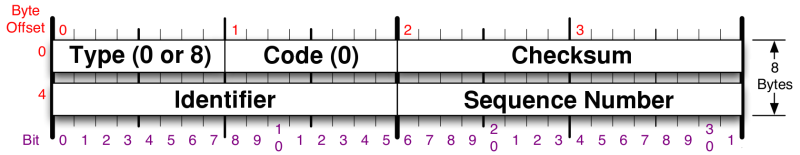
\includegraphics[width=410pt]{../imgs/icmp.png}
\caption{Header de ICMP.}
\end{center}
\end{figure}

\item \textbf{Mensajes de control de ICMP}:
Los mensajes de control que analizaremos a lo largo del trabajo son los siguientes:
\begin{itemize}
\item \textbf{Echo Reply (tipo 0)}: Consiste en un mensaje generado como respuesta a un mensaje Echo Request (petición de Eco).
\item \textbf{Echo Request (tipo 8)}: Consiste en un mensaje de control que se envía a un host con la expectativa de recibir de él un Echo Reply (Respuesta eco).
\item \textbf{Time Exceeded (tipo 11)}: Consiste en un mensaje que se utiliza para indicar que el tiempo de vida de un paquete llegó a su fin.
\end{itemize}

\item \textbf{Round-Trip Time}: Corresponde al retardo del tránsito de paquetes a través de la red IP desde que es enviado hasta volver al emisor, pasando por el destino.

\item \textbf{Traceroute}: Consiste en una herramienta de diagnóstico que muestra la ruta y mide el RTT. Es una herramienta que provee información de cada sistema intermediario (por ejemplo, IPs de routers) que se encuentran a lo largo del camino IP desde el $sender$ hasta el $receiver$. 

\end{itemize}

\section{Desarrollo}
Para la implementación del traceroute, seguimos el siguiente algoritmo:

\begin{algorithm}
\caption{Algoritmo de Traceroute}
\begin{algorithmic}
\Procedure{traceroute}{$IP_{dst}$}

\State $h\gets IP_{dst}$
\State $ttl\gets 1$
\State $anotadas \gets \{\}$
\Repeat
	\State $h.TTL \gets ttl$
	\State $enviar(h, EchoRequest, TimeOut)$
	\If {$obtener(TimeExceeded)\ \&\&\ \neg obtener(TimeOut)$}
    	\State $anotadas.push(IP_{rcv})$
    \Else
    	\State $anotadas.push(^*)$
    \EndIf
    \State $ttl\gets ttl+1$
\Until{$IP_{dst} = IP_{rcv}$}
\EndProcedure
\end{algorithmic}
\end{algorithm}

donde $h$ representa el host destino e $IP_{rcv}$ representa la IP del hop del que proviene el paquete recibido. Por otro lado, $ttl$ representa el \textit{time to live} del paquete y $TTL$ el campo correspondiente en el header del mismo.

El programa comienza enviando mensajes ICMP Echo request con una dirección IP destino y un $Time\ To\ Live$ (TTL) seteado en 1. El primer router que recibe el paquete decrementa el TTL, dado que dicho valor pasa a ser 0, éste descarta el mensaje. Sin embargo, antes de realizar el borrado, el host construye un mensaje de error ICMP (con un mensaje ICMP de tipo ``TTL exceeded'') y lo envía al $sender$. La recepción de dicho mensaje permite al $sender$ identificar qué host se encuentra en un enlace que es camino al destino especificado.

El $sender$ repite el procedimiento dos veces, donde cada una de ellas reporta al host que recibió el paquete. Si todos los paquetes viajan a través del mismo camino, cada mensaje de error ICMP será recibido por el mismo host. En los casos en los que existan dos o más caminos posibles, los resultados pueden variar.

El proceso se repite hasta que el $sender$ recibe una respuesta del destino (o que se alcance el máximo TTL).

Cabe destacar que algunos routers se encuentran configurados para descartar los paquetes ICMP o para procesarlos y no devolver mensajes de error ICMP. Dichos routers ocultan la ``topología'' de la red. Cuando el $traceroute$ se encuentra con un router que no responde, imprime un $^*$.

Para la segunda parte del análisis, modificamos la implementación con el fin de que, una vez terminada la búsqueda, calculara el valor standard o valor Z del RTT (ZRTT) de cada salto $i$ con respecto a la ruta global. Para ello, tuvimos en cuenta las siguientes definiciones:\\

\textit{\textbf{Media:}}
$$\overline{x} = \frac{1}{n} \sum_{i=1}^{n}x_i$$


\textit{\textbf{Desvío standard:}}
$$\sigma = \sqrt{\frac{1}{n} \sum_{i=1}^{n}(x_i - \overline{x})^2}$$

El cambio dio como resultado el siguiente algoritmo:

\begin{algorithm}[H]
\caption{Algoritmo de Traceroute con ZRTT}
\begin{algorithmic}
\Procedure{traceroute}{$IP_{dst}$}

\State $h\gets IP_{dst}$
\State $ttl\gets 1$
\State $anotadas \gets \{\}$
\State $RTTs \gets \{\}$
\Repeat
	\State $h.TTL \gets ttl$
	\State $enviar(h, EchoRequest, TimeOut)$
	\State $clock.reset()$
	\If {$obtener(TimeExceeded)\ \&\&\ \neg obtener(TimeOut)$}
    	\State $anotadas.push(IP_{rcv})$
    \Else
    	\State $anotadas.push(^*)$
    \EndIf
    \State $RTTs_i \gets clock.now()$
    \State $ttl\gets ttl+1$
    \State $ZRTT_i \gets \frac{RTTs_i - promedio(RTTs)}{standDesv(RTTs)}$
\Until{$IP_{dst} = IP_{rcv}$}
\EndProcedure
\end{algorithmic}
\end{algorithm}

Las implementaciones se realizaron en python. Para hallar la ubicación de las direcciones IP utilizamos $pygeoip$. Para ello, fue necesario descargar la base de datos $GeoLiteCity$\footnote{https://code.google.com/p/pysnip/downloads/detail?name=GeoLiteCity.dat} que le asigna una ubicación a cada dirección IP.

Por otro lado, para la construcción de gráficos utilizamos $matplotlib$.

Con el fin de que los resultados fueran variados, elegimos como hosts destino los servidores web de tres universidades ubicadas en continentes distintos.
Las universidades utilizadas fueron:
\begin{itemize}
\item \textbf{University of South Africa}: www.unisa.ac.za\\
Esta universidad se encuentra en Sudáfrica, África.
\item \textbf{University of Zurich}: www.uzh.ch\\
Esta universidad se encuentra en Suiza, Europa.
\item \textbf{International University of Japan}: www.iuj.ac.jp\\
Esta universidad se encuentra en Japón, Asia.
\end{itemize}
\newpage
\section{Resultados}

En primer lugar, decidimos realizar un gráfico de seguimiento de acuerdo a las $longitudes$ y $latitudes$ resultantes del traceroute. Para ello, corrimos el script trace.py con cada sitio web y con un time to live de 30 (por ser el valor TTL máximo utilizado por defecto). Luego, realizamos los gráficos correspondientes.

Por último, realizamos los gráficos correspondientes a las estadísticas pedidas. Éstas son, para cada hop, RTT promedio (el RTT promedio de todos los paquetes recibidos provenientes de ese hop) y ZRTT. Decidimos agregar un umbral para la identificación de enlaces submarinos según los ZRTT relativos obtenidos para cada enlace. El uso de los ZRTT relativos presenta una manera detallada de identificar variaciones de tiempo entre enlaces, pudiendo identificar nodos con una diferencia de RTT mayor al promedio, como tendría un enlace submarino debido a la distancia que recorren los datos. 

Los resultados obtenidos fueron los que siguen:

\subsection{University of South Africa}

\begin{verbatim}
TTL   IP Addresses    Absolute RTT    Relative RTT    Relative ZRTT  Location
1     181.167.145.1      29.022 ms       29.022 ms           -0.056  Argentina
5     200.89.165.57      30.520 ms        1.498 ms           -0.259  Argentina
6     200.89.165.2       29.641 ms       -0.879 ms           -0.290  Argentina
7     200.89.165.86      28.395 ms       -1.247 ms           -0.295  Argentina
8     208.50.25.97       29.425 ms        1.030 ms           -0.265  United States
9     146.82.32.154     285.535 ms      256.110 ms            3.011  United States
10    77.109.128.149    285.473 ms       -0.062 ms           -0.279  Switzerland
11    77.109.128.146    294.840 ms        9.367 ms           -0.158  Switzerland
12    77.109.134.50     244.860 ms      -49.980 ms           -0.920  Switzerland
13    196.32.209.117    425.673 ms      180.813 ms            2.044  South Africa
14    155.232.6.86      432.671 ms        6.998 ms           -0.189  Wynberg, South Africa
15    155.232.6.29      444.425 ms       11.754 ms           -0.128  Wynberg, South Africa
16    155.232.6.138     434.053 ms      -10.372 ms           -0.412  Wynberg, South Africa


\end{verbatim}

\begin{figure}[H] %[h] Aqui [b] para button [t] para top
\begin{center}
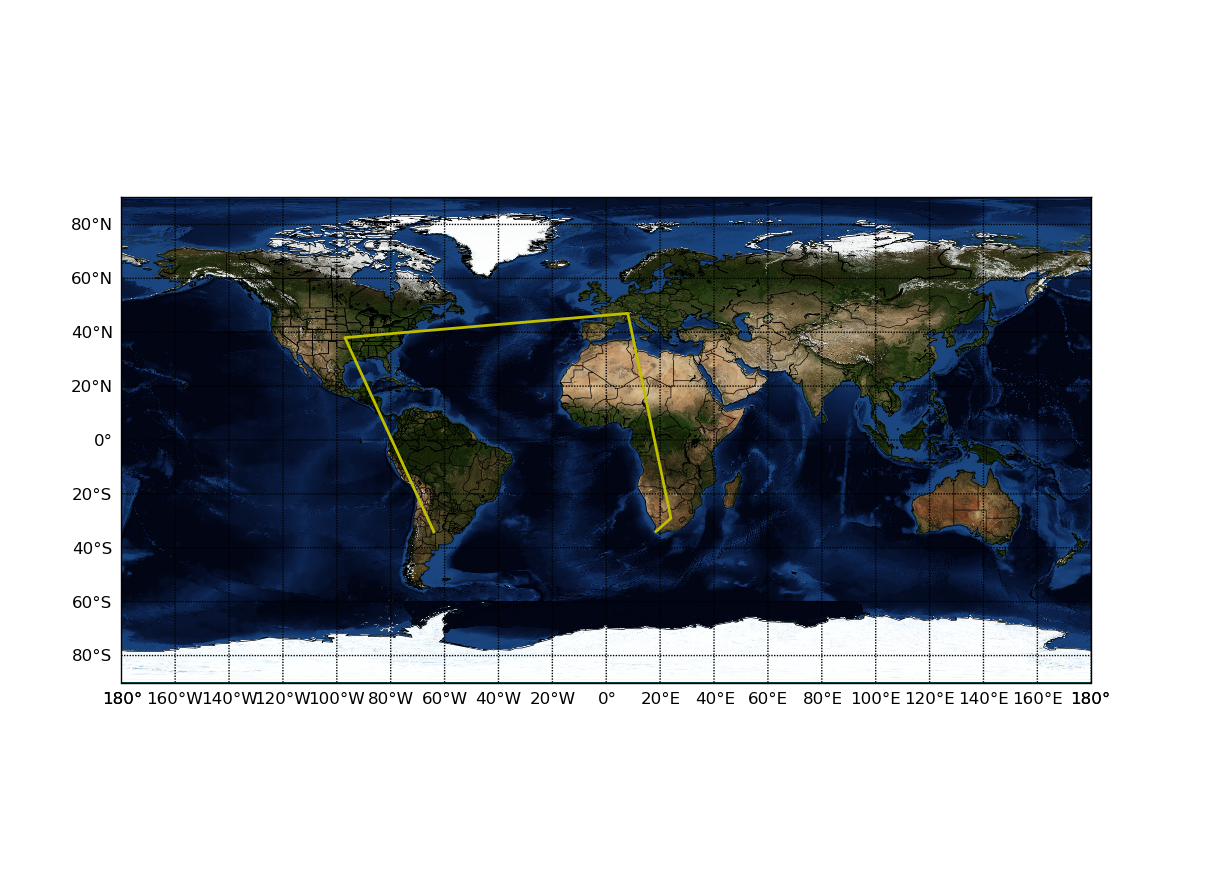
\includegraphics[width=400pt]{../imgs/map-unisa.png}
\caption{Ruta hacia International University of South Africa.}
\end{center}
\end{figure}

%\begin{figure}[H] %[h] Aqui [b] para button [t] para top
%\begin{center}
%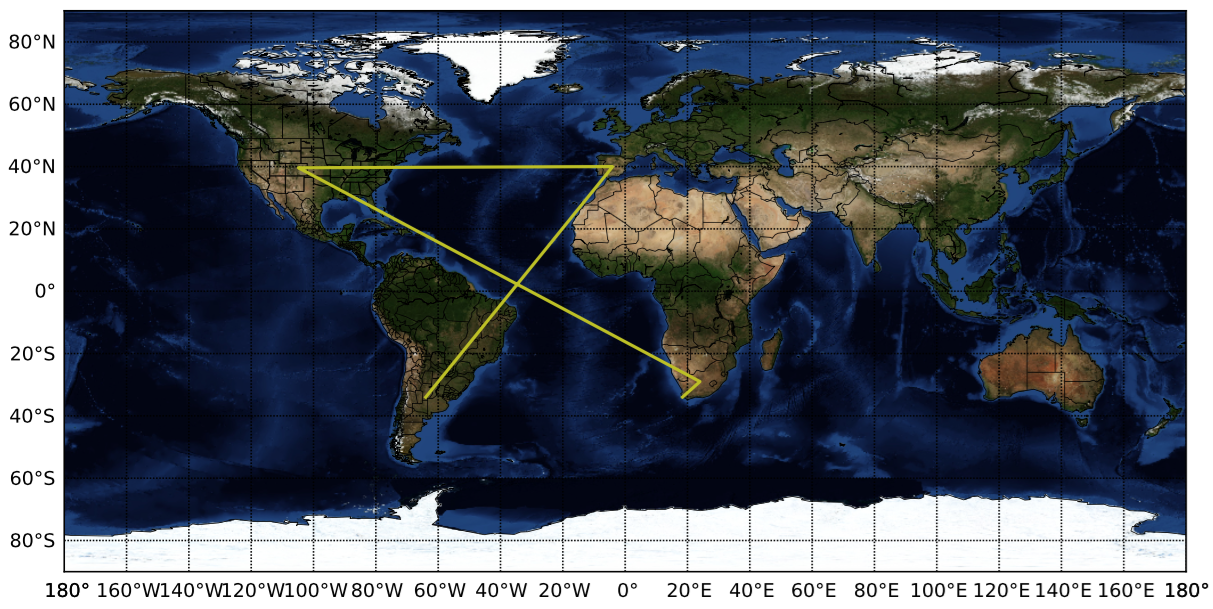
\includegraphics[width=400pt]{../imgs/map-unisa(telef).png}
%\caption{Ruta hacia International University of South Africa desde servicio Telefónica.}
%\end{center}
%\end{figure}

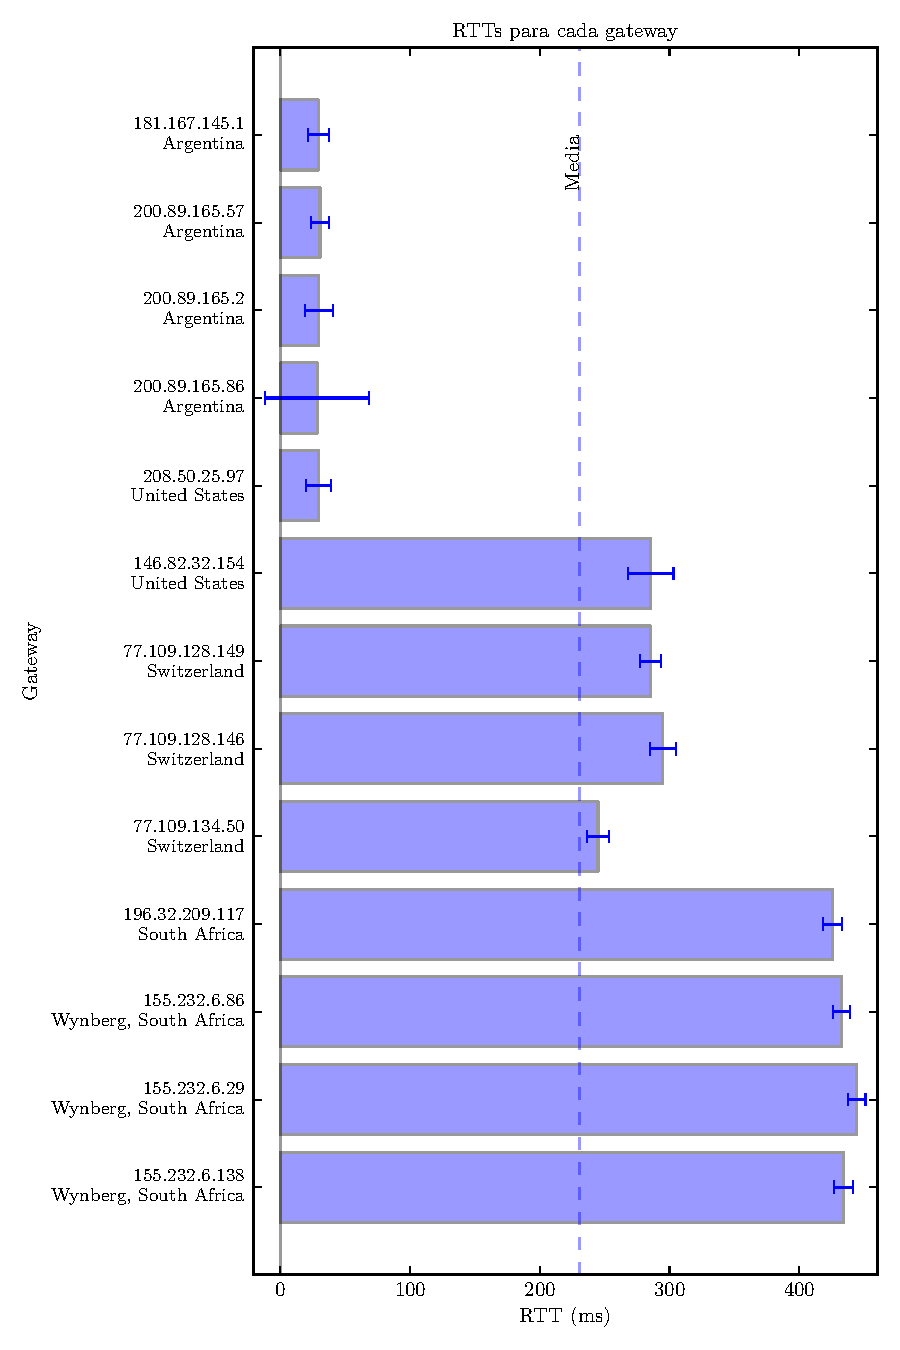
\includepdf[scale=0.70]{../imgs/rtt-unisa.pdf}
En este gráfico podemos ver que el nodo con ip 77.109.134.50 en promedio tarda menos que los 3 nodos que lo anteceden. Este factor suponemos que se da por diferentes rutas en los paquetes, o los nodos anteriores al mismo tienen una baja prioriad para responder paquetes ICMP del tipo Time Exceeded.
También se puede observar el incremento significativo del rtt en en los nodos 146.82.32.154 y 196.32.209.117 con lo que estos podrían ser candidatos a ser tramos finales de los enlaces submarinos. 
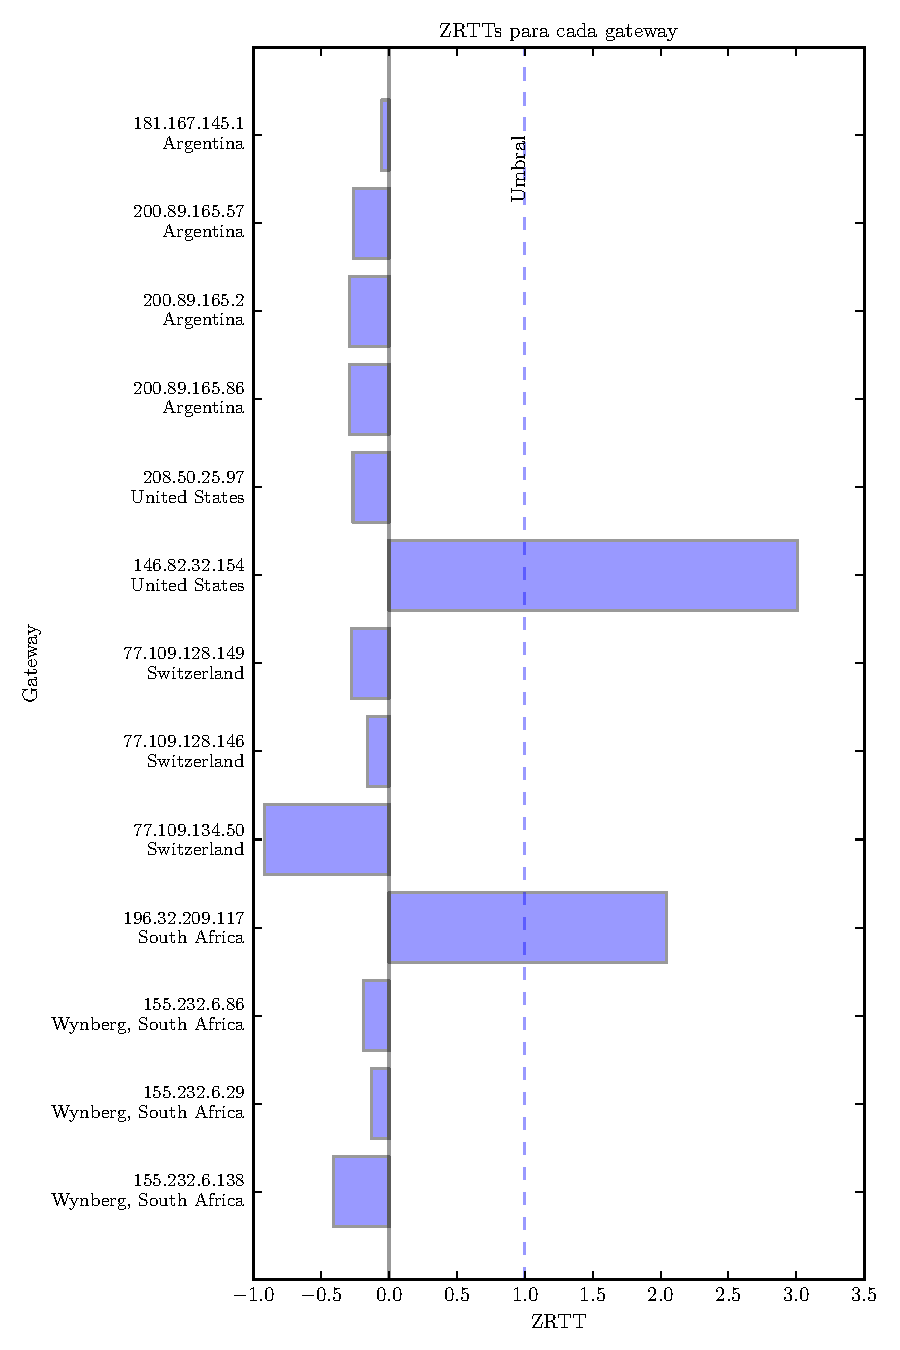
\includepdf[scale=0.70]{../imgs/zrtt-unisa.pdf}

\subsection{University of Zurich}

\begin{verbatim}
TTL   IP Addresses    Absolute RTT    Relative RTT    Relative ZRTT  Location
1     181.167.145.1      27.275 ms       27.275 ms           -0.050  Argentina
5     200.89.165.13      34.171 ms        6.896 ms            0.320  Argentina
6     200.89.165.250     32.573 ms       -1.599 ms            0.250  Argentina
7     208.178.195.205    32.707 ms        0.135 ms            0.265  Alexandria, United States
8     67.17.75.66       167.064 ms      134.356 ms            1.368  United States
9     4.68.111.121      163.154 ms       -3.909 ms            0.231  United States
16    4.69.134.49       297.531 ms      134.377 ms            1.368  United States
17    4.69.137.81       317.171 ms       19.640 ms            0.425  United States
18    213.242.73.74     277.642 ms      -39.529 ms           -0.062  United Kingdom
19    130.59.36.210     295.036 ms       17.394 ms            0.406  Zurich, Switzerland
20    130.59.36.2       269.128 ms      -25.908 ms            0.050  Zurich, Switzerland
21    192.41.136.2      267.857 ms       -1.270 ms            0.253  Zurich, Switzerland
22    192.41.136.71     266.747 ms       -1.110 ms            0.254  Zurich, Switzerland
25    130.60.184.140    268.718 ms        1.971 ms            0.280  Zurich, Switzerland
26    130.60.184.132    263.794 ms       -4.924 ms            0.223  Zurich, Switzerland

\end{verbatim}

\begin{figure}[H] %[h] Aqui [b] para button [t] para top
\begin{center}
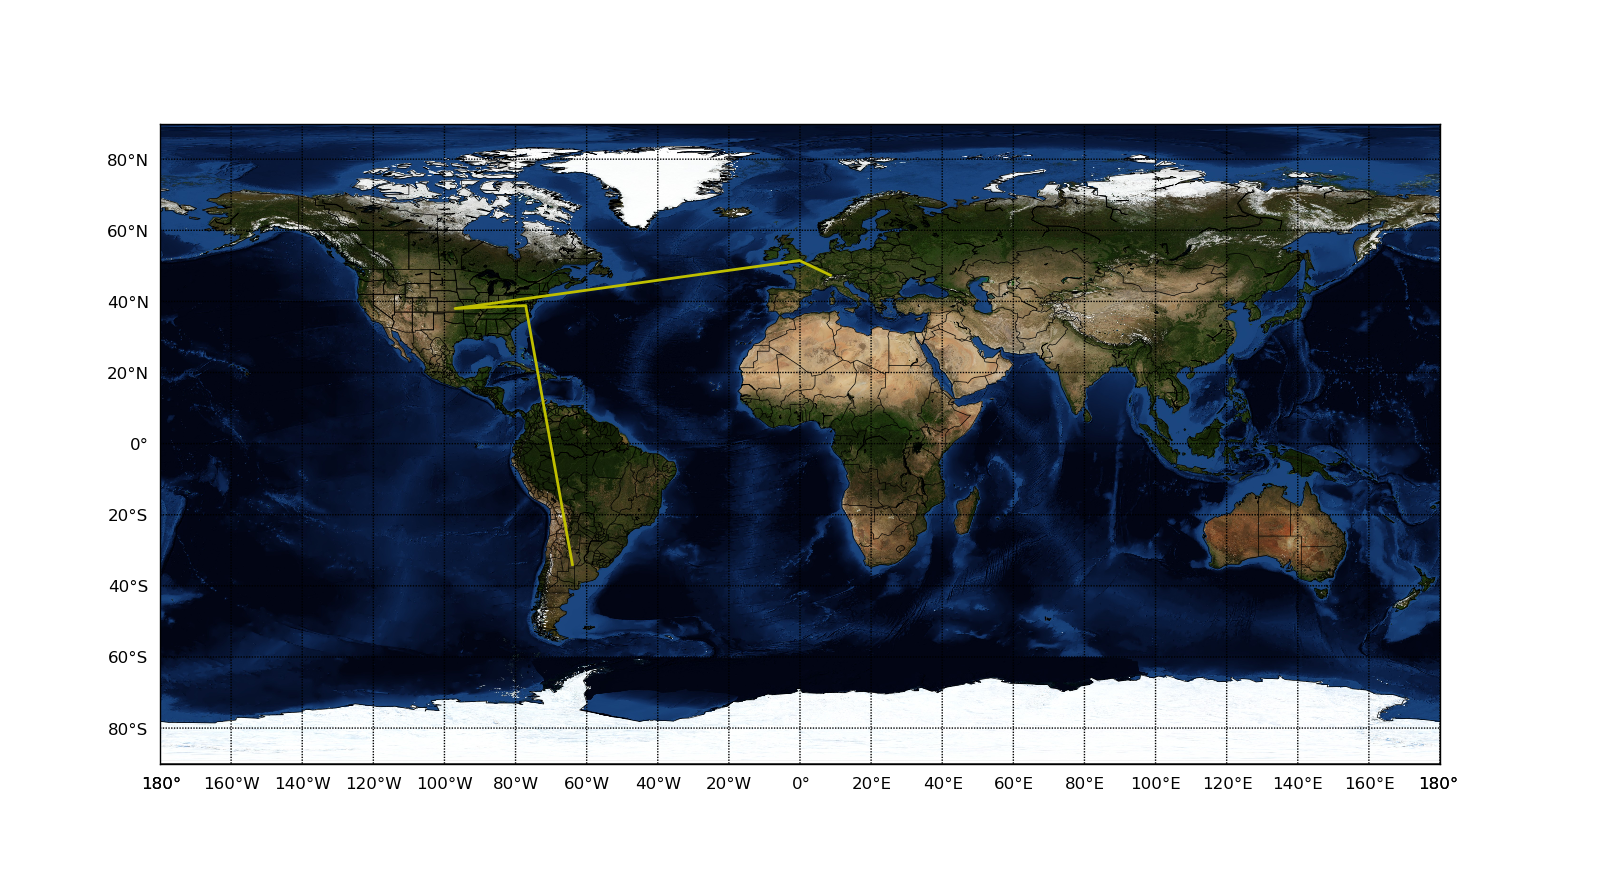
\includegraphics[width=400pt]{../imgs/map-uzh.png}
\caption{Ruta hacia University of Zurich.}
\end{center}
\end{figure}

%\begin{figure}[H] %[h] Aqui [b] para button [t] para top
%\begin{center}
%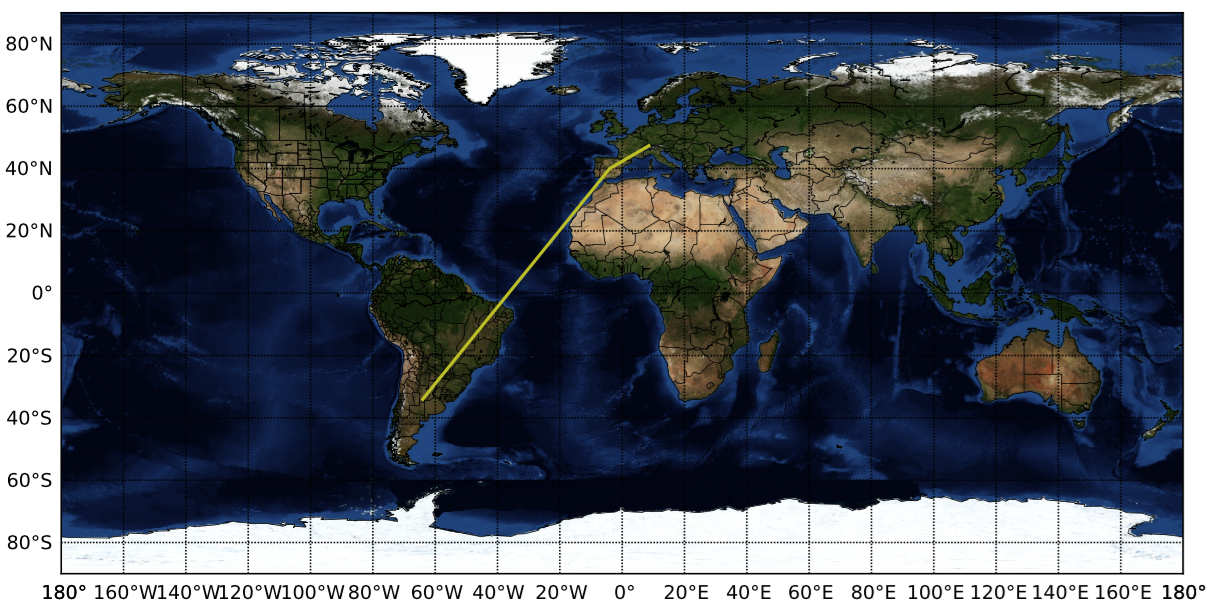
\includegraphics[width=400pt]{../imgs/map-uzh(telef).png}
%\caption{Ruta hacia University of Zurich desde servicio Telefónica.}
%\end{center}
%\end{figure}

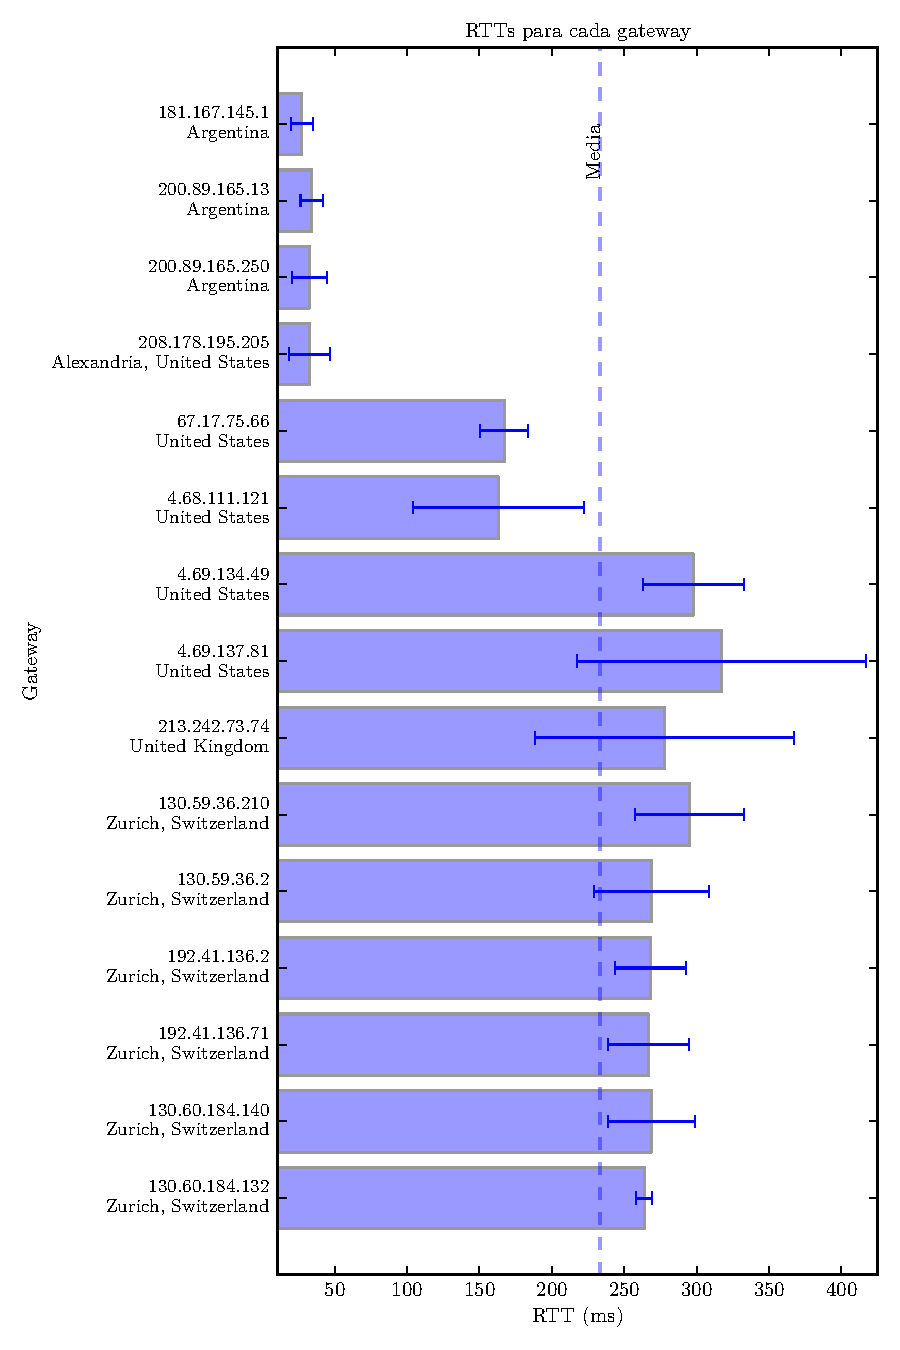
\includepdf[scale=0.70]{../imgs/rtt-uzh.pdf}
En este gráfico podemos ver que algunos nodos tardan menos en promedio que los nodos que lo anteceden. Este factor suponemos que se da por diferentes rutas en los paquetes, o los nodos anteriores al mismo tienen una baja prioriad para responder paquetes ICMP del tipo Time Exceeded.
También se puede observar el incremento significativo del rtt en en los nodos 67.17.75.66 y 4.69.134.49 con lo que estos podrían ser candidatos a ser tramos finales de los enlaces submarinos. 
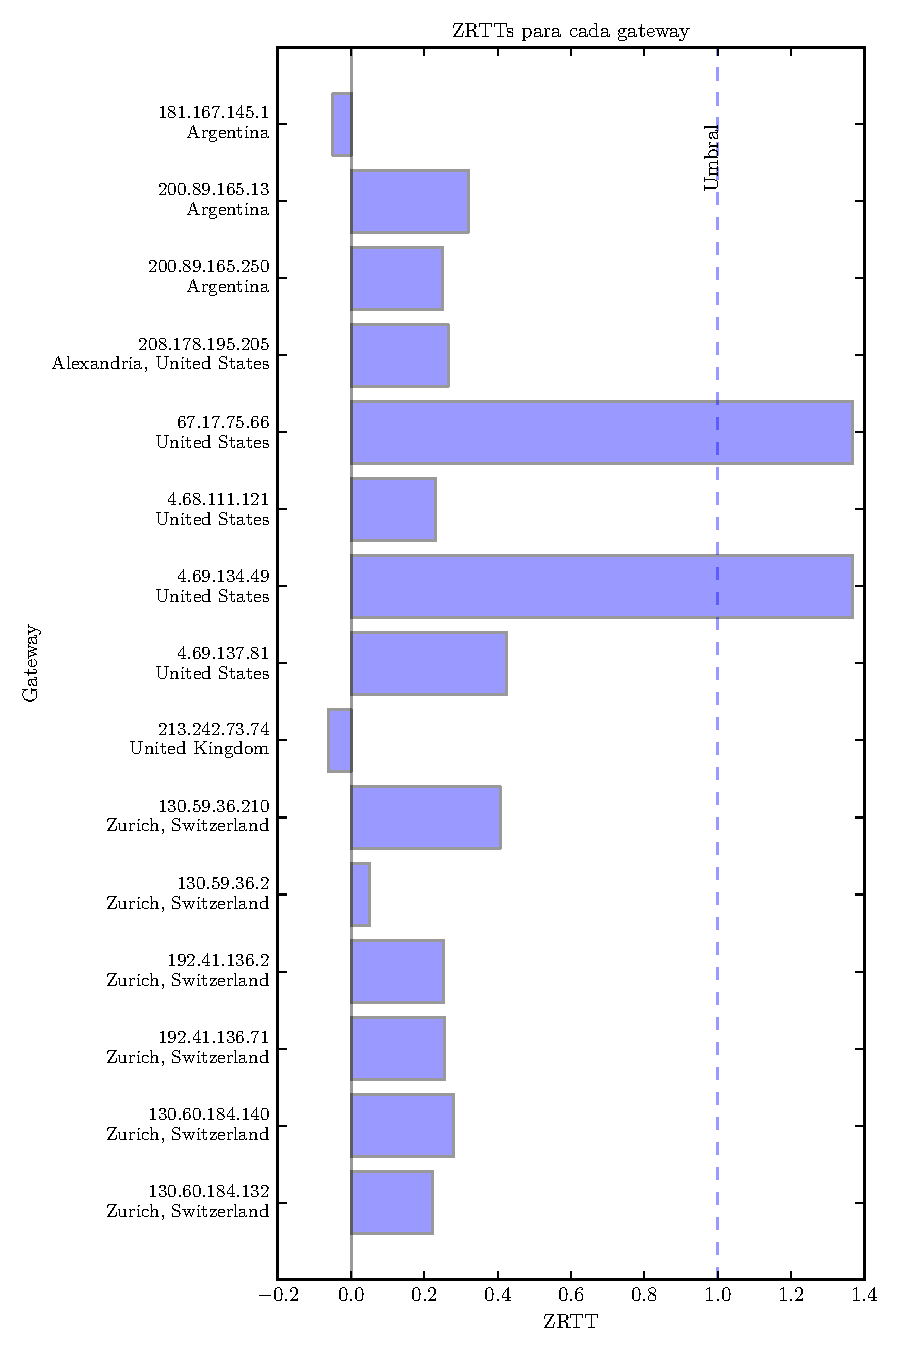
\includepdf[scale=0.70]{../imgs/zrtt-uzh.pdf}
\subsection{International University of Japan}

\begin{verbatim}
TTL   IP Addresses    Absolute RTT    Relative RTT    Relative ZRTT  Location
1     181.167.145.1      45.724 ms       45.724 ms            0.521  Argentina
5     200.89.165.9       38.707 ms       -7.017 ms           -0.362  Argentina
6     200.89.165.250     37.643 ms       -1.064 ms           -0.238  Argentina
7     207.136.166.241    36.375 ms       -1.267 ms           -0.242  United States
8     67.17.106.162     186.092 ms      149.717 ms            2.917  United States
9     64.208.27.102     167.319 ms      -18.774 ms           -0.608  United States
10    129.250.3.172     166.514 ms       -0.804 ms           -0.232  Englewood, United States
11    129.250.3.174     193.829 ms       27.315 ms            0.356  Englewood, United States
12    129.250.2.168     201.637 ms        7.808 ms           -0.052  Englewood, United States
13    129.250.3.15      313.426 ms      111.789 ms            2.124  Englewood, United States
14    129.250.12.198    310.381 ms       -3.045 ms           -0.279  Englewood, United States
15    60.37.27.93       319.185 ms        8.804 ms           -0.031  Japan
16    122.1.246.194     342.279 ms       23.094 ms            0.268  Japan
17    122.28.23.238     334.705 ms       -7.574 ms           -0.374  Japan
18    118.23.5.214      344.825 ms       10.120 ms           -0.004  Japan
19    210.160.35.8      332.892 ms      -11.933 ms           -0.465  Japan
\end{verbatim}

\begin{figure}[H] %[h] Aqui [b] para button [t] para top
\begin{center}
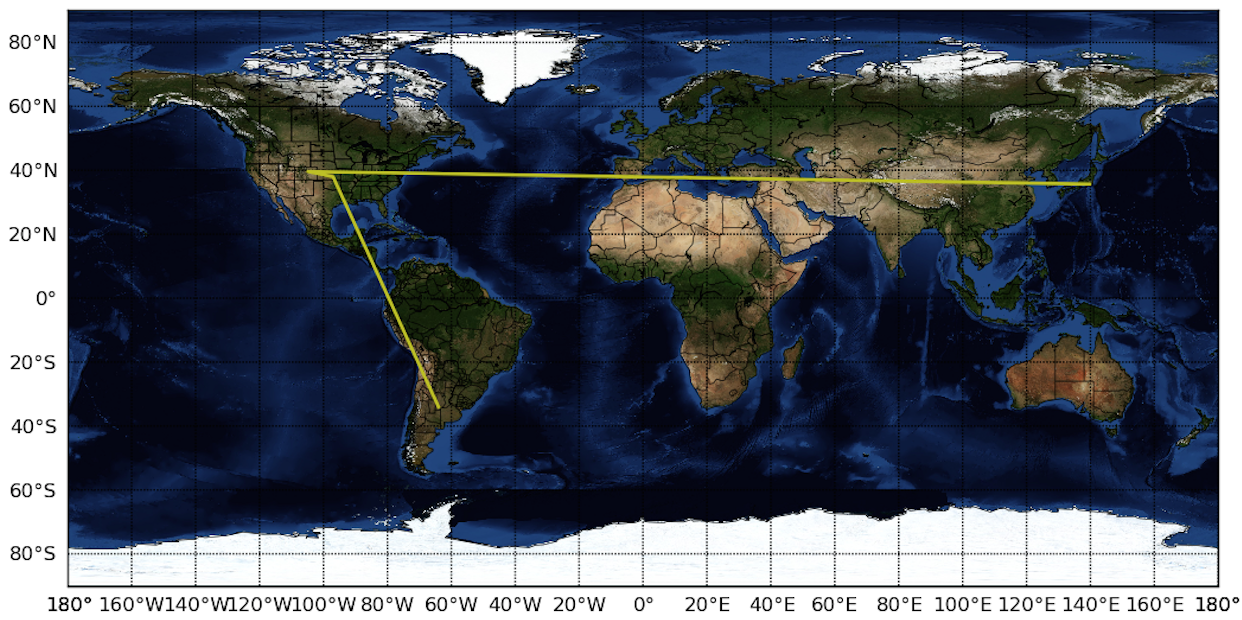
\includegraphics[width=400pt]{../imgs/map-iuj.png}
\caption{Ruta hacia University of Japan.}
\end{center}
\end{figure}

En el mapa anterior, podemos observar que, en primer lugar, la ruta va desde Argentina hacia Estados Unidos. Una vez en allí, podemos percibir que la ruta continúa hacia el centro del país. Si bien el mapa muestra que el enlace atraviesa el Océano Atlántico, suponemos que esto no es más que un error del gráfico dado que la ruta directa hacia Japón atraviesa el Océano Pacífico.

%\begin{figure}[H] %[h] Aqui [b] para button [t] para top
%\begin{center}
%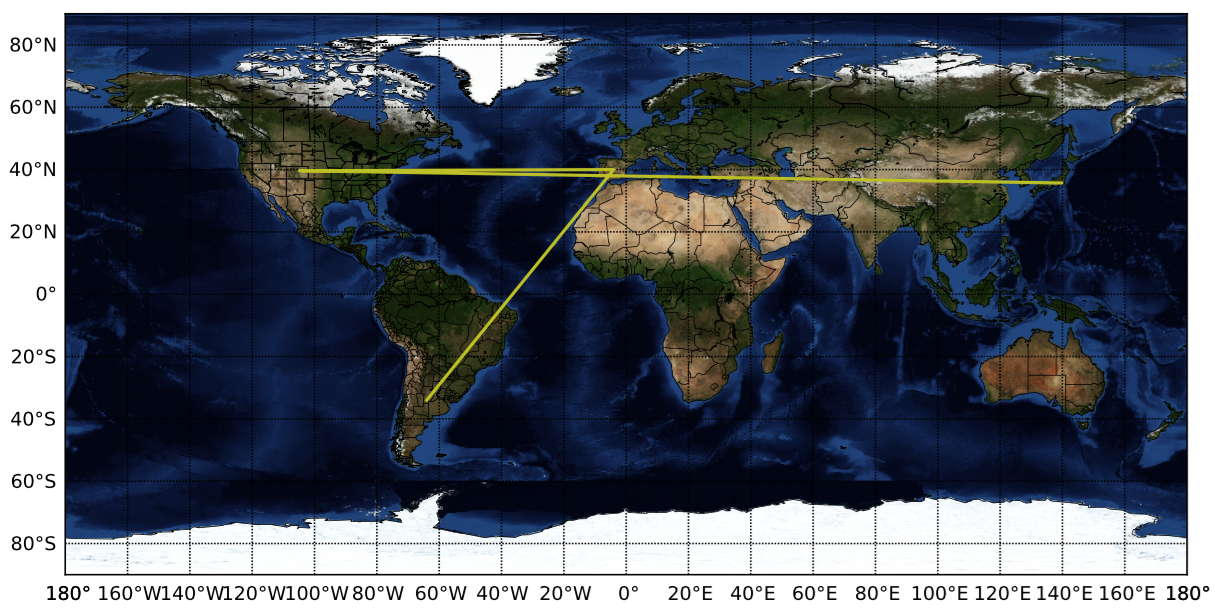
\includegraphics[width=400pt]{../imgs/map-iuj(telef).png}
%\caption{Ruta hacia University of Japan desde servicio Telefónica.}
%\end{center}
%\end{figure}

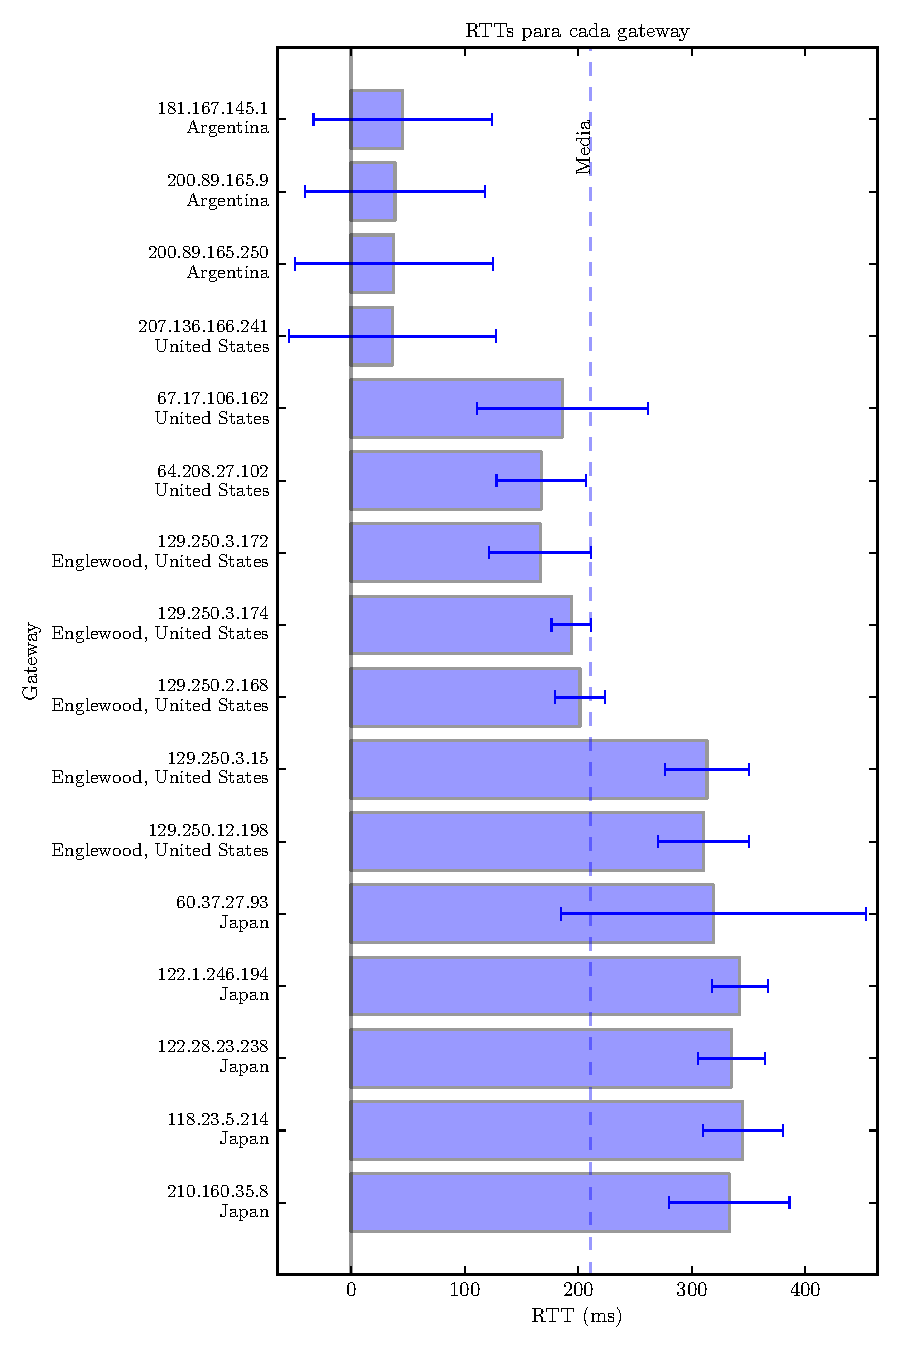
\includepdf[scale=0.70]{../imgs/rtt-iuj.pdf}

En el gráfico anterior, podemos observar que el $RTT$ es bajo para las IPs ubicadas en Argentina, tal como se esperaba. Por otro lado, hallamos un valor bajo en el primer enlace a Estados Unidos (IP 207.136.166.241), lo que nos pareció extraño en comparación con los siguientes valores $RTT$ del mismo país, lo que podría indicar un error de la localización por parte del Geolocalizador. Por último, el $RTT$ a Japón es mayor al de Estados Unidos en pequeña proporción, lo que resultaba esperable.

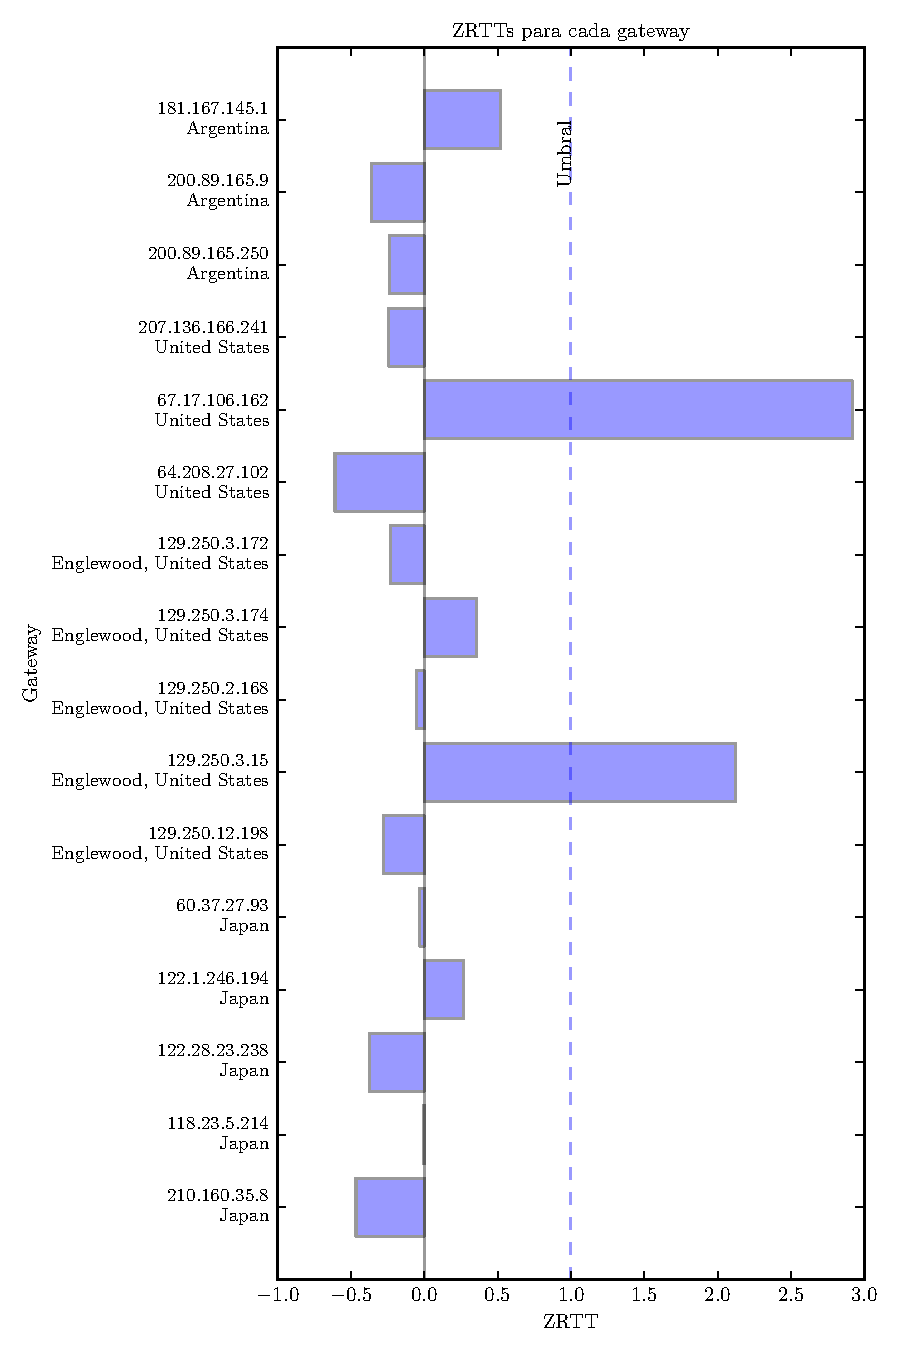
\includepdf[scale=0.70]{../imgs/zrtt-iuj.pdf}
\newpage
\section{Discusión}
Dados los gráficos presentados en la sección anterior, pudimos hallar distintos resultados. 

En primer lugar, pudimos notar que seguramente la empresa que provee los enlaces transatlánticos tenga IPs reservadas y, dado que algunas se encuentran registradas en países que pueden no ser los que poseen dichos hosts físicamente, el geolocalizador le asigne dicha localización. Esta falla se puede ver en la latencia de los saltos dado que en algunos casos, como \textbf{University of Japan}, no tiene sentido que la latencia de Argentina a Estados Unidos sea menor que la de un vínculo interno entre Argentina, siendo este último el lugar de origen.


Por otra parte, notamos que pueden existir distintas rutas posibles hacia un mismo destino, como ya se mencionó anteriormente. Esta particularidad se notó principalmente cuando corrimos el $traceroute$ desde computadoras con distintos servicios de Internet. Veamos el siguiente ejemplo:

\begin{figure}[H] %[h] Aqui [b] para button [t] para top
\begin{center}
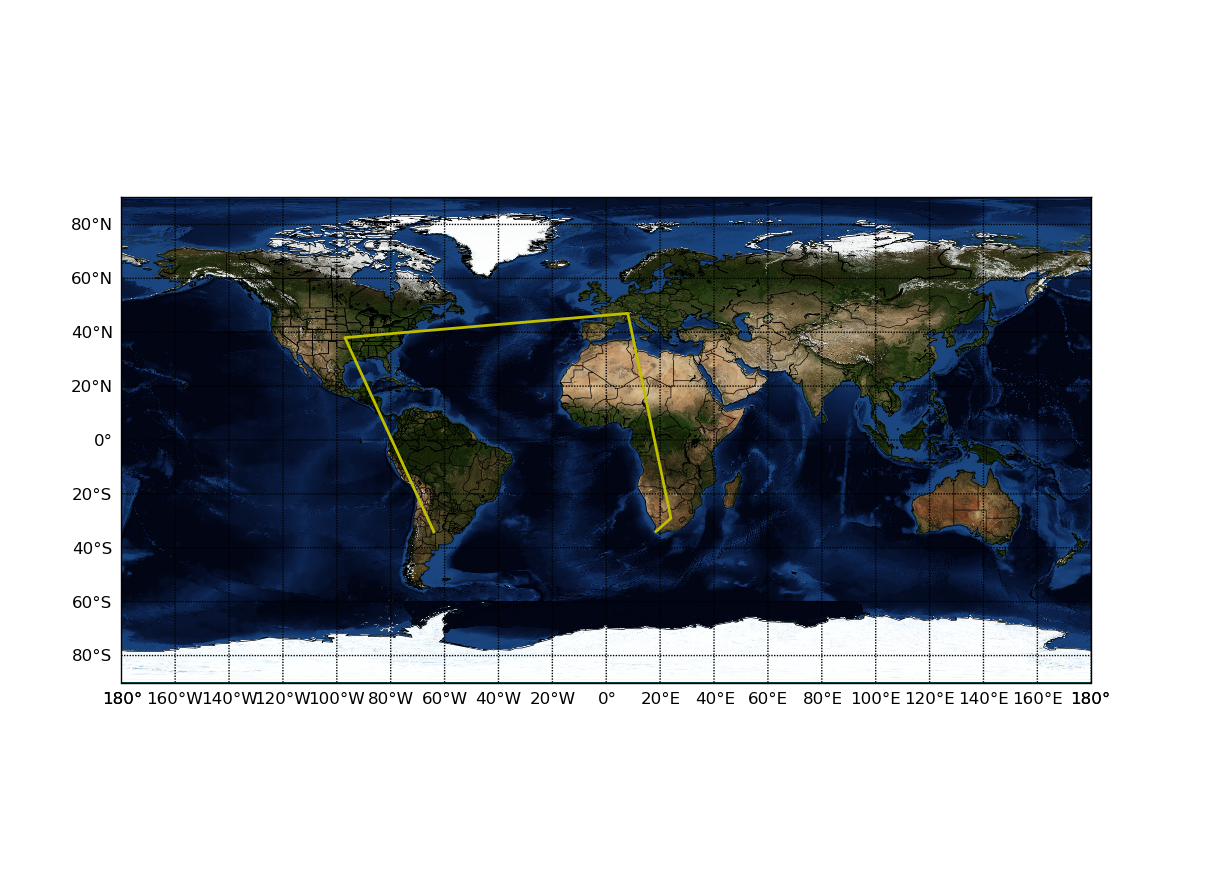
\includegraphics[width=400pt]{../imgs/map-unisa.png}
\caption{Ruta hacia International University of South Africa desde servicio Fibertel.}
\end{center}
\end{figure}

\begin{figure}[H] %[h] Aqui [b] para button [t] para top
\begin{center}
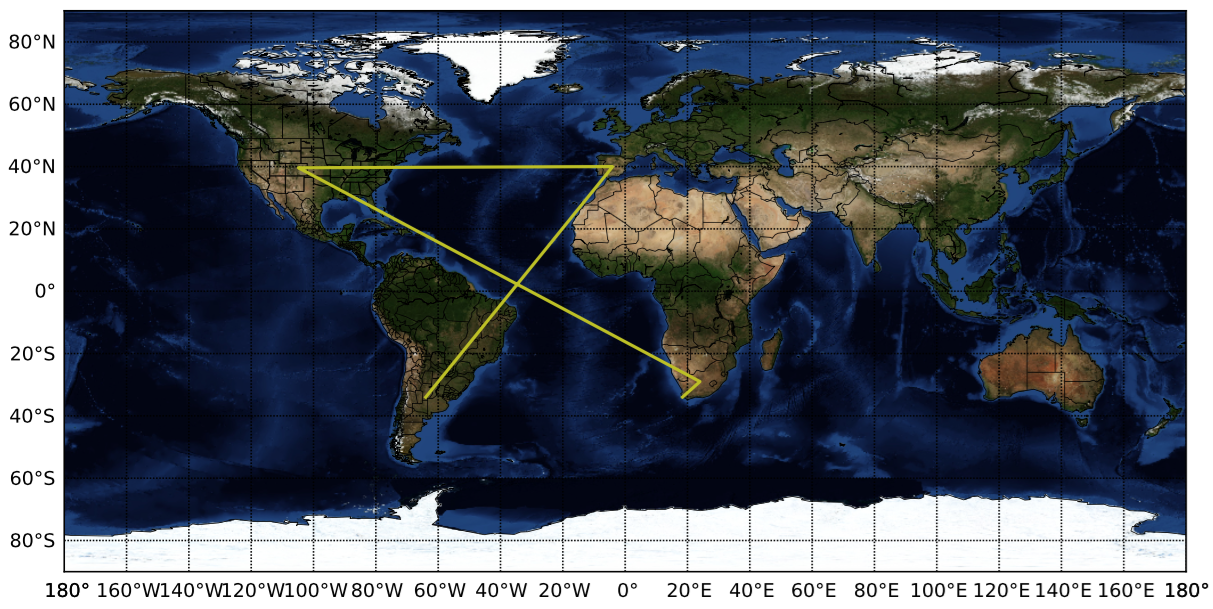
\includegraphics[width=400pt]{../imgs/map-unisa(telef).png}
\caption{Ruta hacia International University of South Africa desde servicio Telefónica.}
\end{center}
\end{figure}

En este caso, podemos notar que el gráfico muestra que la ruta del gateway de \textbf{Telefónica} pasa por España antes de dirigirse a Estados Unidos. Esto puede ocurrir en el caso en el que la IP en cuestión esté registrada por \textbf{Telefónica}, que al ser una empresa española el geolocalizador asocie a dicho país (siendo entonces un posible error del geolocalizador utilizado para las IPs) o porque realmente pase por ese lugar.

Por otro lado, encontramos como anómalo obtener, para un determinado nodo, un RTT absoluto menor al RTT absoluto del nodo anterior, lo que significaría que llegar a este nodo toma menos tiempo que llegar al anterior. Esta anomalía se debe a que los valores del RTT absolutos se calculan mediante el promedio de los RTT obtenidos para cada nodo, pudiendo el paquete ICMP haber tomado caminos diferentes y habiendo conseguido llegar de manera apenas más rápida en promedio. Y además, algunos host podrían darle menos prioridad a responder paquetes ICMP de tipo Time Exceeded que al envío de paquetes al siguiente host.

\subsection{Saltos correspondientes a enlaces submarinos}

En primer lugar, basándonos en el análisis realizado sobre la experimentación, propusimos como umbral en las mediciones de los ZRTT relativos para la detección de enlaces sumbarinos el valor 1. Dicho valor nos pareció suficiente para detectar grandes variaciones en relación al desvío estándar de RTT entre nodos.

Los posibles enlaces submarinos basados en el umbral del ZRTT son:
\begin{itemize}
\item En la traza a la universidad de South Africa hay dos hops que son potenciales enlaces submarinos, estos son el [208.50.25.97(US) - 146.82.32.154(US)] y el [77.109.134.50(SW) - 196.32.209.117(SA)]. Creemos que estos enlaces corresponden a $Argentina \rightarrow EEUU$ y $Suiza \rightarrow Sudafrica$, y la localización dada en el primer hop sea un posible error de la geolocalización.

\item En la traza de la universidad de Zurich los dos hops que se destacan son el [208.178.195.205(US) - 67.17.75.66(US)] y el [4.68.111.121(US) - 4.69.134.49(US)]. En este caso creemos que también se produjo un error en la localización y el primer enlace corresponde a $Argentina \rightarrow EEUU$  y el segundo a $EEUU \rightarrow UK$.

\item En la traza de la universidad de Japón hay dos hops que sobresalen del resto, el [207.136.166.241(US) - 67.17.106.162(US)] y el [129.250.2.168(US) - 129.250.3.15(US)]. En este caso también creemos que es posible que la geolocalización no sea muy precisa y los enlaces correspondan a $Argentina \rightarrow EEUU$ y $EEUU \rightarrow Japon$ respectivamente.
\end{itemize}

\section{Conclusiones}

Concluimos que la técnica estudiada funciona bien en los casos de estudio, sin embargo hay que tener en cuenta que la traza hacia el host destino no posea gateways que demoren más en responder paquetes ICMP de tipo Time Exceeded que lo que demoren en reenviar paquetes al siguiente hop en la ruta a su destino, ya que en esos casos la técnica podría producir falsos positivos.
En el caso general, esta técnica resulta adecuada para identificar hops candidatos a saltos submarinos agregando una etapa de análisis adicional para filtrar los falsos positivos dentro del conjunto de candidatos identificados, de manera de obtener un subconjunto compuesto únicamente por hops correspondientes a saltos submarinos.

\section{Referencias}
\begin{itemize}
\item PETERSON, DAVIE ; Computer Networks, 5th edition, Wiley

\item http://openmaniak.com/ping.php

\item http://www.erg.abdn.ac.uk/~gorry/eg3561/inet-pages/icmp.html
\end{itemize}
\end{document}
